% (c) 2002 Matthew Boedicker <mboedick@mboedick.org> (original author) http://mboedick.org
% % % (c) 2003-2007 David J. Grant <davidgrant-at-gmail.com> http://www.davidgrant.ca
% (c) 2008 Nathaniel Johnston <nathaniel@nathanieljohnston.com> http://www.nathanieljohnston.com
% (l) 2012 Arun I B <arunib@smail.iitm.ac.in> http://www.ee.iitm.ac.in/~ee10s026/
%This work is licensed under the Creative Commons Attribution-Noncommercial-Share Alike 2.5 License. To view a copy of this license, visit http://creativecommons.org/licenses/by-nc-sa/2.5/ or send a letter to Creative Commons, 543 Howard Street, 5th Floor, San Francisco, California, 94105, USA.

\documentclass[letterpaper,11pt]{article}
\newlength{\outerbordwidth}
\pagestyle{empty}
\raggedbottom
\raggedright
\usepackage[svgnames]{xcolor}
\usepackage{framed}
\usepackage{times}
\usepackage{tocloft}
\usepackage{graphicx}
\usepackage{multirow}
\usepackage[utf8]{inputenc}
\usepackage{tabularx}
\usepackage{hyperref}
\usepackage{fancyhdr}
\usepackage{datetime}
\usepackage{fontawesome}
\title{Torsho-CV}

%\fancypagestyle{specialfooter}{%
 % \fancyhf{}
  %\renewcommand\headrulewidth{0pt}
  %\fancyfoot[L]{ \textit{* Minimal working knowledge.}}
%}

\fancypagestyle{latexfooter}{%
  \fancyhf{}
  \renewcommand\headrulewidth{0pt}
  \fancyfoot[R]{\small Page was generated by \LaTeX\ at \today\  \currenttime \  BDT. \href{https://github.com/desertSniper87/official-cv}{\ \color{black}source code: github.com/desertsniper87/official-cv}}
}
%-----------------------------------------------------------
%Edit these values as you see fit

\setlength{\outerbordwidth}{3pt}  % Width of border outside of title bars
\definecolor{shadecolor}{gray}{0.75}  % Outer background color of title bars (0 = black, 1 = white)
\definecolor{shadecolorB}{gray}{0.93}  % Inner background color of title bars


%-----------------------------------------------------------
%Margin setup

\setlength{\evensidemargin}{-0.25in}
\setlength{\headheight}{0in}
\setlength{\headsep}{0in}
\setlength{\oddsidemargin}{-0.25in}
\setlength{\paperheight}{11in}
\setlength{\paperwidth}{8.5in}
\setlength{\tabcolsep}{0in}
\setlength{\textheight}{9.5in}
\setlength{\textwidth}{7in}
\setlength{\topmargin}{-0.3in}
\setlength{\topskip}{0in}
\setlength{\voffset}{0.1in}


%-----------------------------------------------------------
%Custom commands
\newcommand{\resitem}[1]{\item #1 \vspace{-2pt}}
\newcommand{\resheading}[1]{\vspace{8pt}
    \parbox{\textwidth}{\setlength{\FrameSep}{\outerbordwidth}
        \begin{shaded}
            \setlength{\fboxsep}{0pt}\framebox[\textwidth][l]{\setlength{\fboxsep}{4pt}\fcolorbox{shadecolorB}{shadecolorB}{\textbf{\sffamily{\mbox{~}\makebox[6.762in][l]{\large #1} \vphantom{p\^{E}}}}}}
        \end{shaded}
    }\vspace{-5pt}
}
\newcommand{\ressubheading}[4]{
    \begin{tabular*}{6.5in}{l@{\cftdotfill{\cftsecdotsep}\extracolsep{\fill}}r}
        \textbf{#1} & #2 \\
        \textit{#3} & \textit{#4} \\
\end{tabular*}\vspace{-6pt}}
%-----------------------------------------------------------


\begin{document}

%-----------------------------------------------------------
%Insert IIT Madras Logo 
\begin{tabular*}{7in}{l@{\extracolsep{\fill}}r}
  & \multirow{4}{*}[-0.7cm]{
      {
          {%
              \setlength{\fboxsep}{7pt}%
              \setlength{\fboxrule}{0.8pt}%
              \framebox[3.7cm][c]{
              \hspace{-5pt}% add 10pt of horizontal space on the left
              \vspace{0pt}
              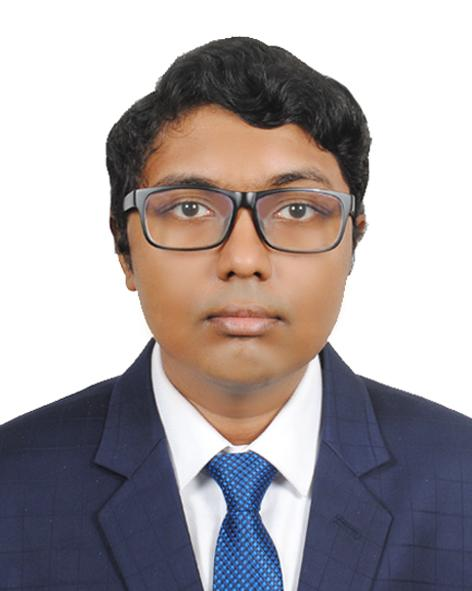
\includegraphics[scale=0.19]{2023-02-23-17-15-39bd847f75daf6f432c82d41c4d76ed6.jpg}}
          }
      }
  }
  & \\
  %-----------------------------------------------------------  
    \textbf{\Large Samidhya Sarker } & \\
    Assistant Programmer & \\
    CA Operations and Security &  \\
    Bangladesh Computer Council & \\
    Infomation and Communication Technology Division & \\
    Ministry of Posts Telecommunications and Information Technology & \\
    Phone: \href{tel:+8801715297522}{\color{black} +8801715297522} \\
    Email: \href{mailto:samidhya.sarker@bcc.gov.bd}{\color{black} samidhya.sarker@bcc.gov.bd} \\
    Links: \href{https://desertsniper87.github.io}{\faHome}\ \href{https://github.com/desertSniper87}{\faGithub}\ \href{https://stackoverflow.com/users/7154462/desertsniper87}{\faStackOverflow}\ \href{https://www.linkedin.com/in/samidhya-sarker-57684275/}{\faLinkedin}
\end{tabular*}
\\


%%%%%%%%%%%%%%%%%%%%%%%%%%%%%%
\resheading{Education}
%%%%%%%%%%%%%%%%%%%%%%%%%%%%%%
\begin{itemize}
    \item
        \ressubheading{Bangladesh University of Engineering and Technology(BUET)}{Dhaka, Bangladesh}{M.Sc. in CSE}{2018 - }
        \begin{itemize}
            \resitem{Postgraduate Thesis: Detection and Recognition of Asymmetric Cartoon Characters in Visual Media}
            \resitem{Advisor: Abu Wasif}
    \end{itemize}
\end{itemize}
\begin{itemize}
    \item
        \ressubheading{Bangladesh University of Engineering and Technology(BUET)}{Dhaka, Bangladesh}{B.Sc. Engineering in CSE}{2011 - 2017}
        \begin{itemize}
            \resitem{Undergraduate Thesis: Efficient Video Transcoding in IaaS Cloud by Using Approximation of Bin-Packing Algorithm in Scheduling.}
            \resitem{Advisor: Dr. S. M. Farhad}
    \end{itemize}
\end{itemize}


%%%%%%%%%%%%%%%%%%%%%%%%%%%%
% \resheading{Personal Statement}
%%%%%%%%%%%%%%%%%%%%%%%%%%%%
% \begin{center}
% \parbox{6.762in}{I am a full stack software developer with an extensive bac}
% \end{center}


%%%%%%%%%%%%%%%%%%%%%%%%%%%%%%
\resheading{Work Experience}
%%%%%%%%%%%%%%%%%%%%%%%%%%%%%%
\begin{itemize}
    \item
        \ressubheading{Bangladesh Computer Council (BCC)}{ICT Division, Dhaka, Bangladesh}{Assistant Programmer, CA Operations and Security}{Dec. 2022 - }
        \begin{itemize}
            \item Currently working as a developer in a  Government Autonomous Institution. 
            \item Working as a frontend (React) developer in Quickpass ios application.
            \item Developed the facematching engine requred for class 2 certificate verification using Machine learning and neural networks and Python frameworks.
            \item Responsible for DevOps of BCC CA internal servers and database servers. 
        \end{itemize}

    \item 
        \ressubheading{BGD e-Gov CIRT}{BCC, ICT Division, Dhaka, Bangladesh}{Quality Assurance (e-Services)}{Dec. 2019 - Dec. 2022}

        \begin{itemize}



            \item Worked as a Software developer/tester in a government project under the umbrella of Bangladesh Computer Council (ICT division), Government of Bangladesh.
            \item I worked as a consultant in the following development teams:
                \begin{enumerate}
                    \item BNDA (Bangladesh National Digital Architecture) Team
                    \item BCC-CA (BCC Certificate Authority) Dev Team
                    \item GRP (Government Resource Planning) BCC Team
                    \item CIRT (Computer Incidence Response Team)
                \end{enumerate}
            \item General responsibilities: 
                \begin{itemize}
                    \item Perform requirement analysis, software specification development,
                        and design software architectures(database, streams etc).
                    \item Development of web application frontends using Angular framework.
                    \item Development of full stack web application using Django/Spring MVC framework.
                    \item Development of web application APIs using django-REST and flask.
                    \item Perorming integration testing, load testing in for web applications.
                    \item Provide training to government employees about developed web applications .
                \end{itemize}

        \end{itemize}

    \item
        \ressubheading{Concitus}{Dhaka, Bangladesh}{Software Engineer}{Oct. 2018 - April. 2019}
        \begin{itemize}
            \item Creating healthcare related web applications Using Python, Django, PostgreSQL, Celery, Redis and VueJS.
            \item Creating Content Management Systems using Django-Wagtail.
        \end{itemize}
\end{itemize}



%%%%%%%%%%%%%%%%%%%%%%%%%%%%%%
\resheading{Skills}
%%%%%%%%%%%%%%%%%%%%%%%%%%%%%%
\begin{itemize}
    \item
        Software Engineering
        \begin{itemize}
            \item {\bf Languages: }{Python, Java, Javascript, C++, C} %Haskell
            \item {\bf Frameworks: }{Django(/REST), FastAPI, Angular, React Native, Celery, Spring MVC/Boot}
            \item {\bf Machine Learning/Data Science: }{{Pytorch, Numpy, Pandas, SciPy, Tensorflow}}
            \item {\bf Database: }{MySQL, PostgreSQL, Redis, SQLite, CockroachDB}
            \item {\bf Mark up/down: }{\LaTeX, {HTML, Markdown, reStructuredText}}
            \item {\bf Func/log prog: }{Clojure, Haskell, Prolog}
            \item {\bf Testing:}{JMeter, Gatling, Cypress, Playright/PuppeteerJS}
            \item {\bf Security Testing:}{Burpsuite, NMap}
                % \item{Server side scripting}{{PHP}}
            \item {\bf Other: }{Git/Mercurial, Vim/Intellij, Postman, Arduino, BeautifulSoup, Scrapy, Selenium, jQuery, Ajax}
        \end{itemize}


    \item
        Systems Operations / DevOps
        \begin{itemize}
            \item{\bf Deployment: }{nGinx/Apache/Tomcat Server administration, Kubernetes/Docker/Dokku/Heroku Deployment Virtualbox/VMware/KVM Deployment}
            \item {Load balancing using Haproxy, nGinx}
            \item {\bf Unix/Linux: }{Distros:
                Debian(Ubuntu), Centos(Fedora), etc.}
            \item Shell Scripting, Ansible 
        \end{itemize}
\end{itemize}


%%%%%%%%%%%%%%%%%%%%%%%%%%%%%%
\resheading{Certification}
%%%%%%%%%%%%%%%%%%%%%%%%%%%%%%
\begin{itemize}
    \item
    \ressubheading{Level-2 Fundamental Information Technology Engineer(ITFE)}{ITPEC, JICA, BCC}{Full Passer}{October 2018}
\end{itemize}


%%%%%%%%%%%%%%%%%%%%%%%%%%%%%%
\resheading{Projects} %%%%%%%%%%%%%%%%%%%%%%%%%%%%%%
\begin{itemize}
\item{\bf It-Connect: }{A helpdesk for aiding ITES development for foreign countries.
    It is a web system developed under the supervision of WB funded LICT-ITES project.
    I designed and developed the frontend of UK and Netherland portal using Angular and parts of the monolithic
    backend using Spring MVC.
    \href{https://bhcl.itconnect.gov.bd}{\ \color{black}[https://bhcl.itconnect.gov.bd]}
    % \href{https://bhcl.itconnect.gov.bd}{\ \color{black}[website]}
}

\item{\bf GRP: }{Government Resource Planning application of Government of Bangladesh.
    I worked at the frontend of the Payment submodule of the HRM module which is responsible for disbursing the
    salary of GoB employees.
    \href{https://grp.gov.bd}{\ \color{black}[https://grp.gov.bd]}
    % \href{https://grp.gov.bd}{\ \color{black}[website]}
}

\item{\bf HIS: }{Health Information System application of BCC.
    I designed and developed the web application using Django, MySQL. 
    \href{https://his.bcc.gov.bd}{\ \color{black}[https://his.bcc.gov.bd]}
    % \href{https://his.bcc.gov.bd}{\ \color{black}[website]}
}

\item{\bf e-Recruitment: }{Recruitment system of BCC.
    I performed, load/stress testing, automated UI functionality testing, integration testing
    and server administration.
    % \href{https://erecruitment.bcc.gov.bd}{\ \color{black}[website]}
    \href{https://erecruitment.bcc.gov.bd}{\ \color{black}[https://erecruitment.bcc.gov.bd]}
}

\item{\bf Boithok: }{Video conferencing system of ICTD.
    I performed, load/stress testing, functionality testing of the system and the android
    application.  
    \href{https://vc.bcc.gov.bd}{\ \color{black}[https://vc.bcc.gov.bd]}
    % \href{https://vc.bcc.gov.bd}{\ \color{black}[website]}
}

\item{\bf Covid19Tracker: }{Covid19 Tracker application developed by BNDA. 
    I developed the analytics dashboard using d3js.
    \href{http://covid19tracker.gov.bd/}{\ \color{black}[http://covid19tracker.gov.bd]}
    % \href{http://covid19tracker.gov.bd/}{\ \color{black}[website]}
}

\item{\bf FPS: }{Foodgrain Procurement System of Food Department of GoB. 
    I performed load/stress testing, UI testing.
    \href{http://fps.dgfood.gov.bd/}{\ \color{black}[http://fps.dgfood.gov.bd]}
    % \href{http://fps.dgfood.gov.bd/}{\ \color{black}[website]}
}
\end{itemize}


%%%%%%%%%%%%%%%%%%%%%%%%%%%%%%
\resheading{Communication Skills}
%%%%%%%%%%%%%%%%%%%%%%%%%%%%%%
\begin{itemize}
\item{\bf Bangla: }{Native Language}
\item{\bf English: }{Full Professional Proficiency}
\item{\bf German: }{Limited Working Proficiency}
\end{itemize}


%%%%%%%%%%%%%%%%%%%%%%%%%%%%%%
\resheading{Co-curricular activities}
%%%%%%%%%%%%%%%%%%%%%%%%%%%%%%
\begin{itemize}
\item{16 times blood donor for Badhan.}
\item{Volunteer, BUET CSE Festival 2011, 2013, 2015 Inter University Project Show (IUPS)}
% \item{Contributor, Bengali Language Wikipedia \href{https://bn.wikipedia.org/wiki/User:Desertsniper87}{\color{black}[profile]}}
\item{Contributor, Bengali Language Wikipedia \href{https://bn.wikipedia.org/wiki/User:Desertsniper87}{\color{black}[https://bn.wikipedia.org/wiki/User:Desertsniper87]}}
\end{itemize}


%%%%%%%%%%%%%%%%%%%%%%%%%%%%%%
\resheading{Reference}
%%%%%%%%%%%%%%%%%%%%%%%%%%%%%%
\begin{itemize}
    \item Abu Wasif \hfill \break
          Assistant Professor \hfill \break
          ECE Building, Room No. 403, BUET \hfill \break
          Email: \href{mailto:wasif@cse.buet.ac.bd}{\color{black} wasif@cse.buet.ac.bd}
\end{itemize}


\thispagestyle{latexfooter}

\end{document}
